
\documentclass[%
 reprint,
%superscriptaddress,
%groupedaddress,
%unsortedaddress,
%runinaddress,
%frontmatterverbose, 
%preprint,
%preprintnumbers,
nofootinbib,
%nobibnotes,
%bibnotes,
 amsmath,amssymb,
 aps,
%pra,
%prb,
%rmp,
%prstab,
%prstper,
floatfix,
]{revtex4-2}
\usepackage{gensymb}
\usepackage{textcomp}
\usepackage{lipsum}
\usepackage{graphicx}% Include figure files
\usepackage{dcolumn}% Align table columns on decimal point 


\usepackage{bm}% bold math
\usepackage{siunitx}
\DeclareSIUnit\gauss{G}
\DeclareSIUnit\erg{erg}
\DeclareMathOperator{\Rot}{rot}
\sisetup{separate-uncertainty=true}
\usepackage{tabularx}
\usepackage{amssymb}
\usepackage{amsmath}
\usepackage{relsize}
\usepackage{commath}
\usepackage{enumitem}
\usepackage{xfrac}
\usepackage{float}
\usepackage{booktabs}
\usepackage{makecell}
\usepackage{caption}
\usepackage{subcaption}
\usepackage{multirow}
\usepackage[version=4]{mhchem}
\usepackage[colorlinks,bookmarks=false,citecolor=blue,linkcolor=blue,urlcolor=blue]{hyperref}
%\usepackage{hyperref}% add hypertext capabilities
%\usepackage[mathlines]{lineno}% Enable numbering of text and display math
%\linenumbers\relax % Commence numbering lines

%\usepackage[showframe,%Uncomment any one of the following lines to test 
%%scale=0.7, marginratio={1:1, 2:3}, ignoreall,% default settings
%%text={7in,10in},centering,
%%margin=1.5in,
%%total={6.5in,8.75in}, top=1.2in, left=0.9in, includefoot,
%%height=10in,a5paper,hmargin={3cm,0.8in},
%]{geometry}

\begin{document}

\preprint{APS/123-QED}

\title{Rutherford Scattering}% Force line breaks with \\


\author{Maitrey Sharma}
\email{maitrey.sharma@niser.ac.in}
\affiliation{School of Physical Sciences, National Institute of Science Education and Research, HBNI, Jatni-752050, India}




\date{\today}% It is always \today, today,
             %  but any date may be explicitly specified

\begin{abstract}
    In this experiment, we perform the famous Gold foil experiment whose results were first explained by Ernest Rutherford in 1909. We bombard Gold (and later Aluminium) foil by using a alpha source Am-241 and observe the scattering that happens at various angles (orientations) between the source beam and the receiving foil. We explain the results so obtained and compare them from Gold and Aluminium foils. We also determine the atomic number of Aluminium.
\end{abstract}

\keywords{}
\maketitle

%\tableofcontents

\section{\label{sec:level1}Introduction}
    In 1909, Hans Geiger and Ernest Marsden performed the gold foil experiment in collaboration with Ernest Rutherford, in which they fired a beam of alpha particles (helium nuclei) at foils of gold leaf only a few atoms thick. At the time of the experiment, the atom was thought to be analogous to a plum pudding (as proposed by J. J. Thomson), with the negatively-charged electrons (the plums) studded throughout a positive spherical matrix (the pudding). If the plum-pudding model were correct, the positive "pudding", being more spread out than in the correct model of a concentrated nucleus, would not be able to exert such large coulombic forces, and the alpha particles should only be deflected by small angles as they pass through.
    \par
    However, the intriguing results showed that around 1 in 20,000 alpha particles were deflected by very large angles (over 90°), while the rest passed through with little deflection. From this, Rutherford concluded that the majority of the mass was concentrated in a minute, positively-charged region (the nucleus) surrounded by electrons. When a (positive) alpha particle approached sufficiently close to the nucleus, it was repelled strongly enough to rebound at high angles. The small size of the nucleus explained the small number of alpha particles that were repelled in this way. Rutherford showed, using the method outlined below, that the size of the nucleus was less than about $10^{-14}$ m (how much less than this size, Rutherford could not tell from this experiment alone; see more below on this problem of lowest possible size). As a visual example, figure (\ref{fig:cloudchamber}) shows the deflection of an alpha particle by a nucleus in the gas of a cloud chamber.
    \begin{figure}
        \centering
        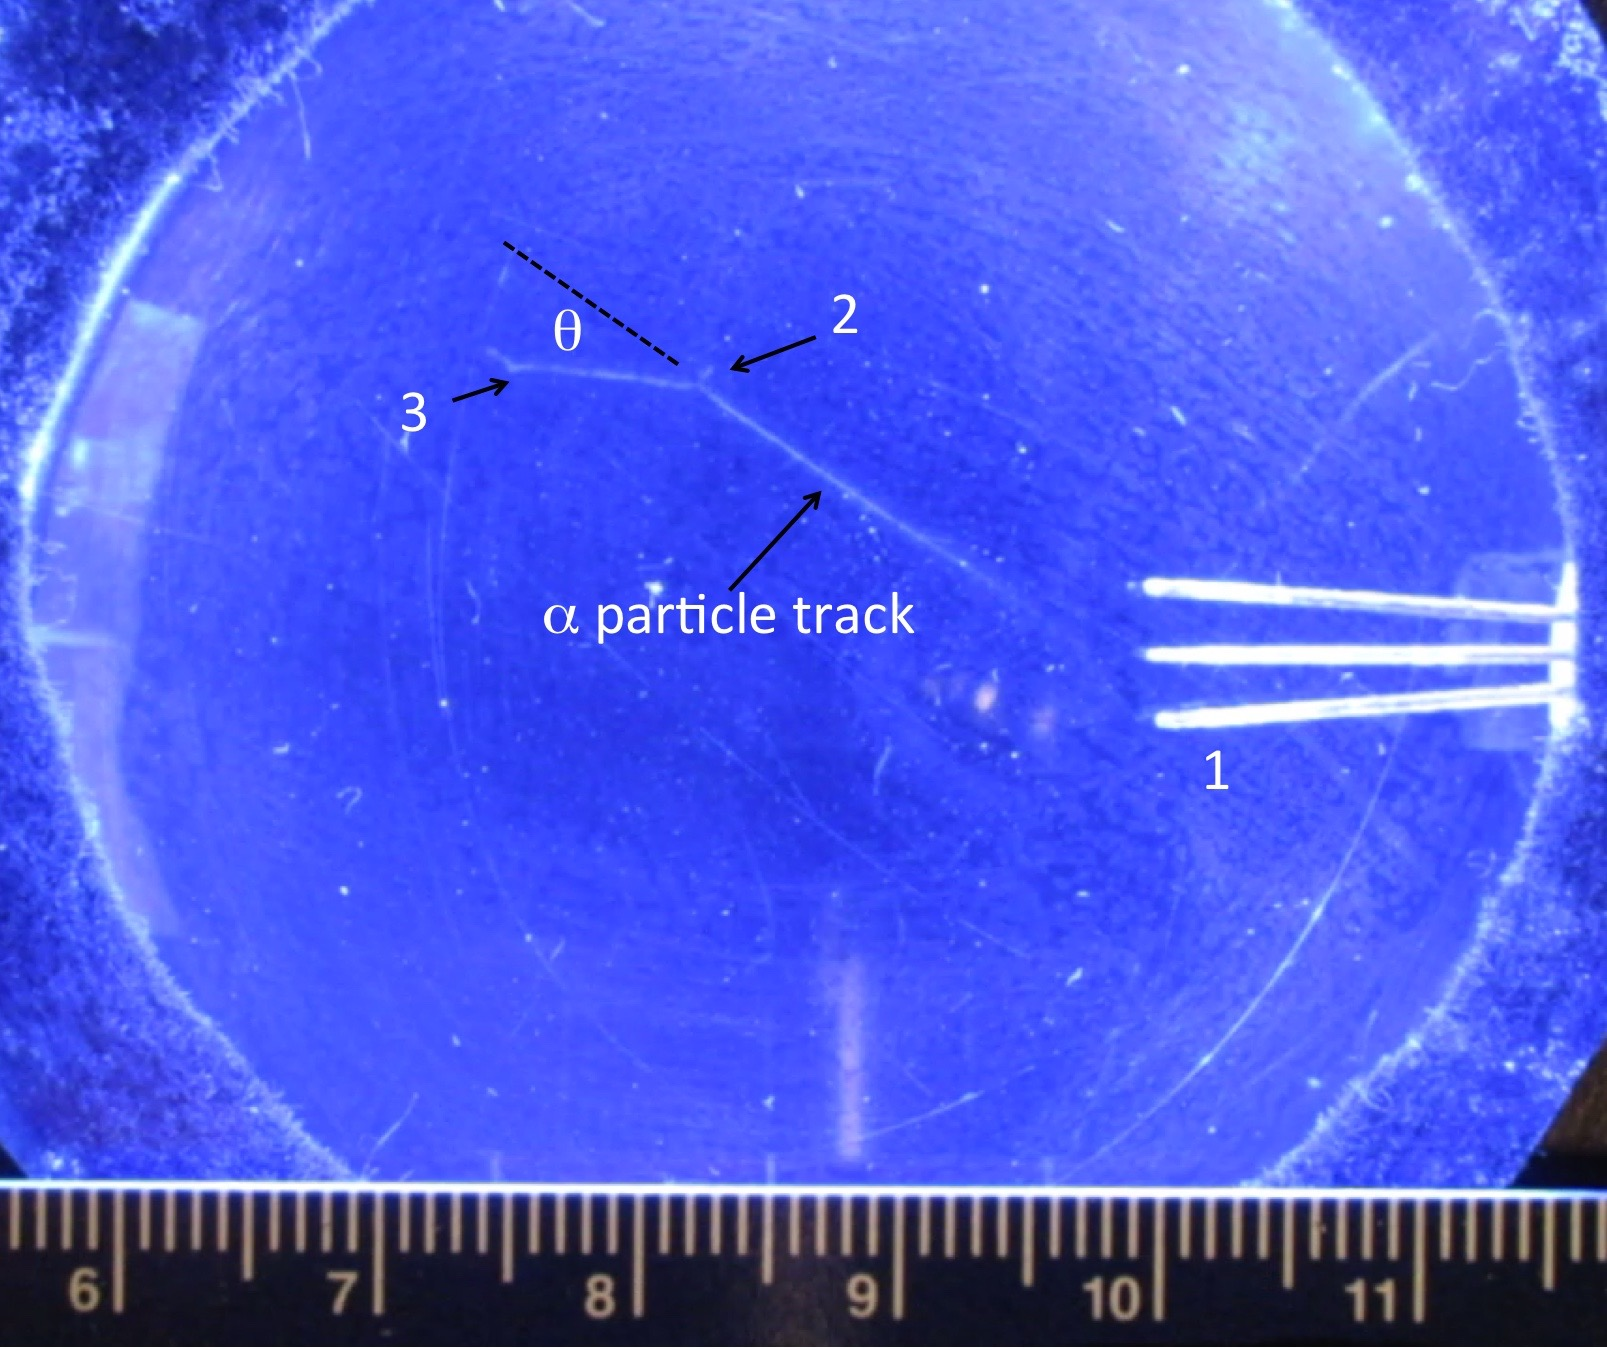
\includegraphics[scale = 0.15]{Figures/AlphaTrackRutherfordScattering3.jpg}
        \caption{In a cloud chamber, a $\SI{5.3}{\mega \electronvolt}$ alpha particle track from a lead-210 pin source near point 1 undergoes Rutherford scattering near point 2, deflecting by an angle of about $30 \degree$. It scatters once again near point 3, and finally comes to rest in the gas. The target nucleus in the chamber gas could have been a nitrogen, oxygen, carbon, or hydrogen nucleus. It received enough kinetic energy in the elastic collision to cause a short visible recoiling track near point 2. (The scale is in centimeters.)}
        \label{fig:cloudchamber}
    \end{figure}
    \par
    Rutherford scattering is the elastic scattering of charged particles by the Coulomb interaction. It led to the development of the planetary Rutherford model of the atom and eventually the Bohr model. Rutherford scattering was first referred to as Coulomb scattering because it relies only upon the static electric (Coulomb) potential, and the minimum distance between particles is set entirely by this potential. The classical Rutherford scattering process of alpha particles against gold nuclei is an example of \textit{elastic scattering} because neither the alpha particles nor the gold nuclei are internally excited.
    
    
\section{Apparatus}
\begin{enumerate}
    \item Scattering chamber after Rutherford
    \item Aluminium and Gold foil in frame
    \item Vacuum pump
    \item Discriminator preamplifier
    \item Counter
    \item Plug-in power supply unit
    \item Am-241 preparation
\end{enumerate}

\section{Experiment description}
    The experimental appratues is given in figure (\ref{fig:setup})
    \begin{figure}
        \centering
        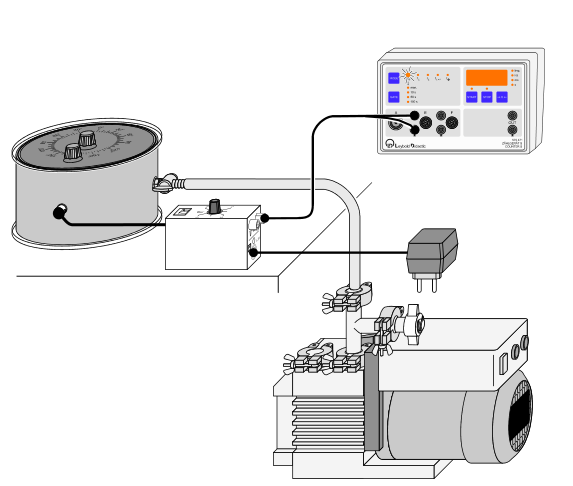
\includegraphics[scale = 0.5]{Figures/setup.png}
        \caption{Experimental setup schematically for the Rutherford Scattering Experiment.}
        \label{fig:setup}
    \end{figure}
    The detailed diagram of the scattering chamber is given in figure (\ref{fig:chamber}).
    \begin{figure}
        \centering
        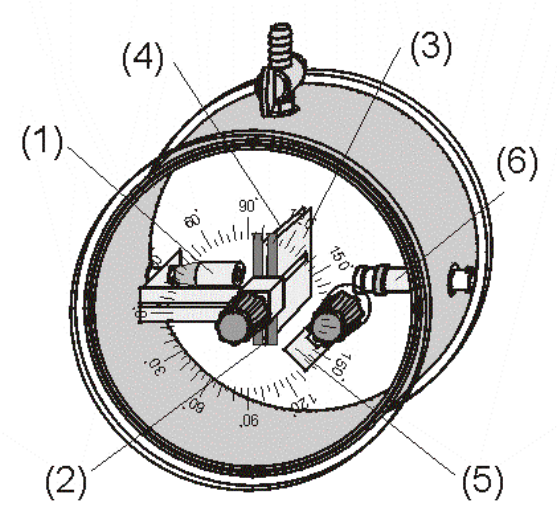
\includegraphics[scale = 0.6]{Figures/chamber.png}
        \caption{The scattering chamber (1) Preparation (2) Holder (3) Gold foil (4) Slit (5) swivel arm (6) detector}
        \label{fig:chamber}
    \end{figure}
    The scattering geometry is given in figure (\ref{fig:geometry}).
    \begin{figure}
        \centering
        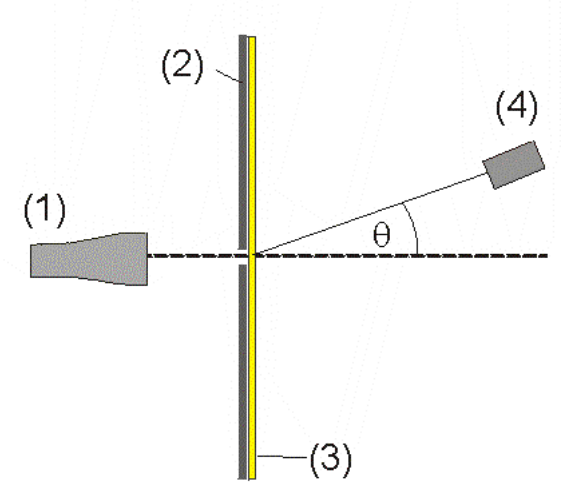
\includegraphics[scale = 0.6]{Figures/geometry.png}
        \caption{The scattering geometry (1) preparation (2) collimator slit (3) gold foi (4) detector}
        \label{fig:geometry}
    \end{figure}
    

\section{Theory}
    If $\alpha$-particles are allowed to strike a thin gold foil, they are deflected from their path (\textit{scattering}), each by an angle $\theta$. The majority of $\alpha$-particles is scattered by angles less than $1 \degree$ (figure (\ref{fig:scattering})).
    \begin{figure}
        \centering
        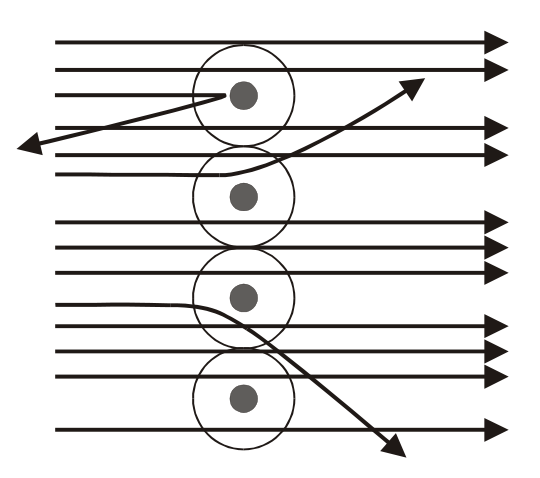
\includegraphics[scale = 0.6]{Figures/scattering.png}
        \caption{Scattering of $\alpha$-particles on a monolayer of atoms.}
        \label{fig:scattering}
    \end{figure}
    \par
    A few particles, however, show substantially large scattering angles $\theta$, in the extreme case up to $180 \degree$ (\textit{back scattering}). These initially qualitative observations can only be explained by assuming that the gold atoms have a very small nucleus, containing practically the whole atomic mass, and being positively charged.
    \par
    On the basis of this idea Rutherford calculated the angular distribution of the scattering rate $N(\theta)$. The scattering rate is the number of particles which are scattered during the time unit in a determined interval $d \theta$ around an average angle $\theta$. The result of this calculation is \textit{Rutherford’s scattering formula}:
    \begin{equation}
    \label{eq:Ntheta}
        N (\theta) = N_0 \cdot c_F \cdot d_F \dfrac{Z^2 \cdot d^4}{(8 \pi \epsilon_0 E_{\alpha})^2 \cdot \sin^4 (\theta/2)}
    \end{equation}
    where $N_0$ is the particle rate in the foil; $c_F$ is the atomic concentration in the foil; $d_F$ is the thickness of the foil; $Z$ is the nuclear charge number of the scattering material; $E_{\alpha}$ is the energy of the $\alpha$-particles; $e$ is the elementary charge ($e = \SI{1.6021e-19}{\ampere \second}$); $\epsilon_0$ is the dielectric constant in vacuum ($\epsilon_0 = \SI{8.8524e-12}{\ampere \second \per \volt \per \metre}$).
    \par
    The $\alpha$-particles emitted from the Am-241 preparation fall through a slit aperture of $\SI{5}{\milli \metre}$ width onto the gold foil and leave this gold foil with various scattering angles. The scattered $\alpha$-particles are identified with a semiconductor detector.
    \par
    If we compare the scattering rates between two different foil materials (e.g. Au and Al) at the same angle $\theta$, we can derive from the scattering formula (\ref{eq:Ntheta}):
    \begin{equation}
        \dfrac{N_{Au}}{N_{Al}} = \dfrac{c_{Au} d_{Au} Z^2_{Au}}{c_{Al} d_{Al} Z^2_{Al}}
    \end{equation}
    and thus
    \begin{equation}
    \label{eq:Zal}
        Z_{Al} = \sqrt{\dfrac{N_{Al}(\theta) c_{Au} d_{Au} Z^2_{Au}}{N_{Au}(\theta) c_{Al} d_{Al}}}
    \end{equation}


    
    
\section{Evaluation and Results}
    After recording the pulse counts $n(\theta)$ the mean values $n_m(\theta)$ can be determined. Using the mean values $n_m(\theta)$ the scattering rates $N_d(\theta)$ are calculated by
    \begin{equation}
        N_d(\theta) = \dfrac{n_m (\theta)}{t(\theta)}
    \end{equation}
    These measuring results $N_d(\theta)$ are typical for a plane scattering geometry which is given by the transparent construction of the chamber used in this experiment. The theoretical function (according to Rutherford’s formula), however, is related to a three-dimensional geometry. The relation between these different aspects can considered by the following concept (figure (\ref{fig:angle})).
    \begin{figure}
        \centering
        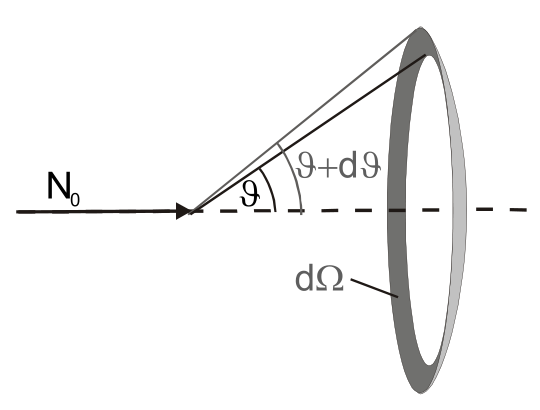
\includegraphics[scale = 0.7]{Figures/angular.png}
        \caption{The $\alpha$-particles are scattered into the angular region $\vartheta + d \vartheta$.}
        \label{fig:angle}
    \end{figure}
    \par
    Each plane angle $\theta$ corresponds in space to a cone with an aperture of $2 \cdot \theta$ (produced by rotation of the plane structure around the incident beam axis). In the same way the plane angular differential $d \theta$ corresponds in three dimensions to a spatial angular differential $d \Omega$ given by
    \begin{equation}
        d \Omega = 2 \cdot \pi \cdot \sin (\theta) d\theta 
    \end{equation}
    This geometrical corrections allows to derive a relation between the plane scattering rate $N_d(\theta)$ and the spatial scattering rate $N(\theta)$:
    \begin{equation}
        N (\theta) = 2 \cdot \pi \cdot \sin (\theta) \cdot N d\theta 
    \end{equation}
    Finally, the corresponding spatial values $N(\theta)$ are calculated (\ref{tab:data}) and the space corrected values plotted in a diagram (\ref{fig:graph}).
    \par
    The measuring value pairs $\{\theta / N(\theta )\}$ can be compared with the shape of the theoretical curve of equation:
    \begin{equation}
        f(\theta) = \dfrac{A}{\sin^4 \Big( \dfrac{\theta - b}{2} \Big)}
    \end{equation}
    The proportionality factor $A$ represents a vertical shift (at logarithmic scale). The coefficient $B$ is representing a small displacement along the horizontal angular scale.
    \par
    Now we have for $N_{Au} (15 \degree) = \SI{18.701}{\per \second} $ and $N_{Al} (15 \degree) = \SI{3.402}{\per \second}$ with $d_{Au} = \SI{2}{\micro \metre}$, $d_{Al} = \SI{8}{\micro \metre}$, $c_{Au} \approx c_{Al}$ and $Z_{Au} = 79$, we obtain from equation (\ref{eq:Zal}):
    \begin{equation}
        Z_{Al} = 16.8
    \end{equation}
    and for $N_{Au} (-15 \degree) = \SI{4.011}{\per \second} $ and $N_{Al} (-15 \degree) = \SI{0.285}{\per \second}$ and rest of the parameters same as before, we get
    \begin{equation}
        Z_{Al} = 10.5
    \end{equation}
    Taking mean $Z_{Al}$, we obtain $Z_{Al} = 13.7$ which is close to the actual value of $Z_{Al} = 13$.
    \par
    The data recorded is tabulated in table (\ref{tab:data}). The corresponding plot between scattering angle $\theta$ and $N(\theta)$ is given in figure (\ref{fig:graph}).
    \newcommand{\ra}[1]{\renewcommand{\arraystretch}{#1}}
    \begin{table*}[]
    \ra{1.2}
    \caption{Measured values for Gold foil and slit width $d = \SI{5}{\milli \metre}$}
    \label{tab:data}
    \setlength{\tabcolsep}{5pt}
    \begin{tabular}{@{}ccccccc@{}}
    \toprule
    \begin{tabular}[c]{@{}c@{}}\textbf{Angle}, $\theta$\\ (degrees)\end{tabular} & \begin{tabular}[c]{@{}c@{}}\textbf{Angle}, $\theta$\\ (radians)\end{tabular} & \begin{tabular}[c]{@{}c@{}}\textbf{Gate time} $t(\theta)$\\ ($\si{\second}$)\end{tabular} & \textbf{Pulse counts} $n(\theta)$ & \begin{tabular}[c]{@{}c@{}}\textbf{Mean Pulse counts}\\ $n_m(\theta)$ \end{tabular} & \begin{tabular}[c]{@{}c@{}}\textbf{Counting rate} \\ \textit{(directly)} \\ $N_d (\theta)$ ($\si{\per \second}$)\end{tabular} & \begin{tabular}[c]{@{}c@{}}\textbf{Counting rate} \\ \textit{(space corrected)} \\ $N (\theta)$ ($\si{\per \second}$)\end{tabular} \\ \midrule
    \multirow{3}{*}{-30}                                    & \multirow{3}{*}{-0.524}                                        & \multirow{3}{*}{900}                                    & 148          & \multirow{3}{*}{152}                                                 & \multirow{3}{*}{0.169}                                              & \multirow{3}{*}{0.531}                                                            \\
                                                            &                                                                &                                                         & 151          &                                                                      &                                                                     &                                                                                   \\
                                                            &                                                                &                                                         & 157          &                                                                      &                                                                     & \\                                                                                   \\
    \multirow{3}{*}{-25}                                    & \multirow{3}{*}{-0.436}                                        & \multirow{3}{*}{600}                                    & 227          & \multirow{3}{*}{230}                                                 & \multirow{3}{*}{0.383}                                              & \multirow{3}{*}{1.016}                                                            \\
                                                            &                                                                &                                                         & 241          &                                                                      &                                                                     &                                                                                   \\
                                                            &                                                                &                                                         & 221          &                                                                      &                                                                     &  \\                                                                                 \\
    \multirow{3}{*}{-20}                                    & \multirow{3}{*}{-0.349}                                        & \multirow{3}{*}{200}                                    & 572          & \multirow{3}{*}{594}                                                 & \multirow{3}{*}{2.970}                                              & \multirow{3}{*}{6.382}                                                            \\
                                                            &                                                                &                                                         & 597          &                                                                      &                                                                     &                                                                                   \\
                                                            &                                                                &                                                         & 613          &                                                                      &                                                                     &   \\                                                                                \\
    \multirow{3}{*}{-15}                                    & \multirow{3}{*}{-0.262}                                        & \multirow{3}{*}{100}                                    & 1181         & \multirow{3}{*}{1150}                                                & \multirow{3}{*}{11.500}                                             & \multirow{3}{*}{18.701}                                                           \\
                                                            &                                                                &                                                         & 1126         &                                                                      &                                                                     &                                                                                   \\
                                                            &                                                                &                                                         & 1143         &                                                                      &                                                                     &  \\                                                                                 \\
    \multirow{3}{*}{-10}                                    & \multirow{3}{*}{-0.175}                                        & \multirow{3}{*}{100}                                    & 2797         & \multirow{3}{*}{2817}                                                & \multirow{3}{*}{28.173}                                             & \multirow{3}{*}{30.739}                                                           \\
                                                            &                                                                &                                                         & 2771         &                                                                      &                                                                     &                                                                                   \\
                                                            &                                                                &                                                         & 2884         &                                                                      &                                                                     &   \\                                                                                \\
    -5                                                      & -0.087                                                         & 100                                                     & 3558         & 3558                                                                 & 35.580                                                              & 19.484                                                                            \\ \\
    5                                                       & 0.087                                                          & 100                                                     & 2787         & 2787                                                                 & 27.870                                                              & 15.262                                                                            \\ \\
    \multirow{3}{*}{10}                                     & \multirow{3}{*}{0.175}                                         & \multirow{3}{*}{100}                                    & 1204         & \multirow{3}{*}{1246}                                                & \multirow{3}{*}{12.460}                                             & \multirow{3}{*}{13.595}                                                           \\
                                                            &                                                                &                                                         & 1265         &                                                                      &                                                                     &                                                                                   \\
                                                            &                                                                &                                                         & 1269         &                                                                      &                                                                     &  \\                                                                                 \\
    \multirow{3}{*}{15}                                     & \multirow{3}{*}{0.262}                                         & \multirow{3}{*}{100}                                    & 246          & \multirow{3}{*}{247}                                                 & \multirow{3}{*}{2.467}                                              & \multirow{3}{*}{4.011}                                                            \\
                                                            &                                                                &                                                         & 255          &                                                                      &                                                                     &                                                                                   \\
                                                            &                                                                &                                                         & 239          &                                                                      &                                                                     &  \\                                                                                  \\
    \multirow{3}{*}{20}                                     & \multirow{3}{*}{0.349}                                         & \multirow{3}{*}{200}                                    & 86           & \multirow{3}{*}{75}                                                  & \multirow{3}{*}{0.375}                                              & \multirow{3}{*}{0.806}                                                            \\
                                                            &                                                                &                                                         & 71           &                                                                      &                                                                     &                                                                                   \\
                                                            &                                                                &                                                         & 68           &                                                                      &                                                                     &   \\                                                                                \\
    \multirow{3}{*}{25}                                     & \multirow{3}{*}{0.436}                                         & \multirow{3}{*}{600}                                    & 104          & \multirow{3}{*}{115}                                                 & \multirow{3}{*}{0.192}                                              & \multirow{3}{*}{0.509}                                                            \\
                                                            &                                                                &                                                         & 128          &                                                                      &                                                                     &                                                                                   \\
                                                            &                                                                &                                                         & 113          &                                                                      &                                                                     &   \\                                                                                \\
    \multirow{3}{*}{30}                                     & \multirow{3}{*}{0.524}                                         & \multirow{3}{*}{900}                                    & 77           & \multirow{3}{*}{73}                                                  & \multirow{3}{*}{0.081}                                              & \multirow{3}{*}{0.254}                                                            \\
                                                            &                                                                &                                                         & 72           &                                                                      &                                                                     &                                                                                   \\
                                                            &                                                                &                                                         & 69           &                                                                      &                                                                     &   \\                                                                                 \bottomrule
    \end{tabular}
    \end{table*}
    \begin{figure}
        \centering
        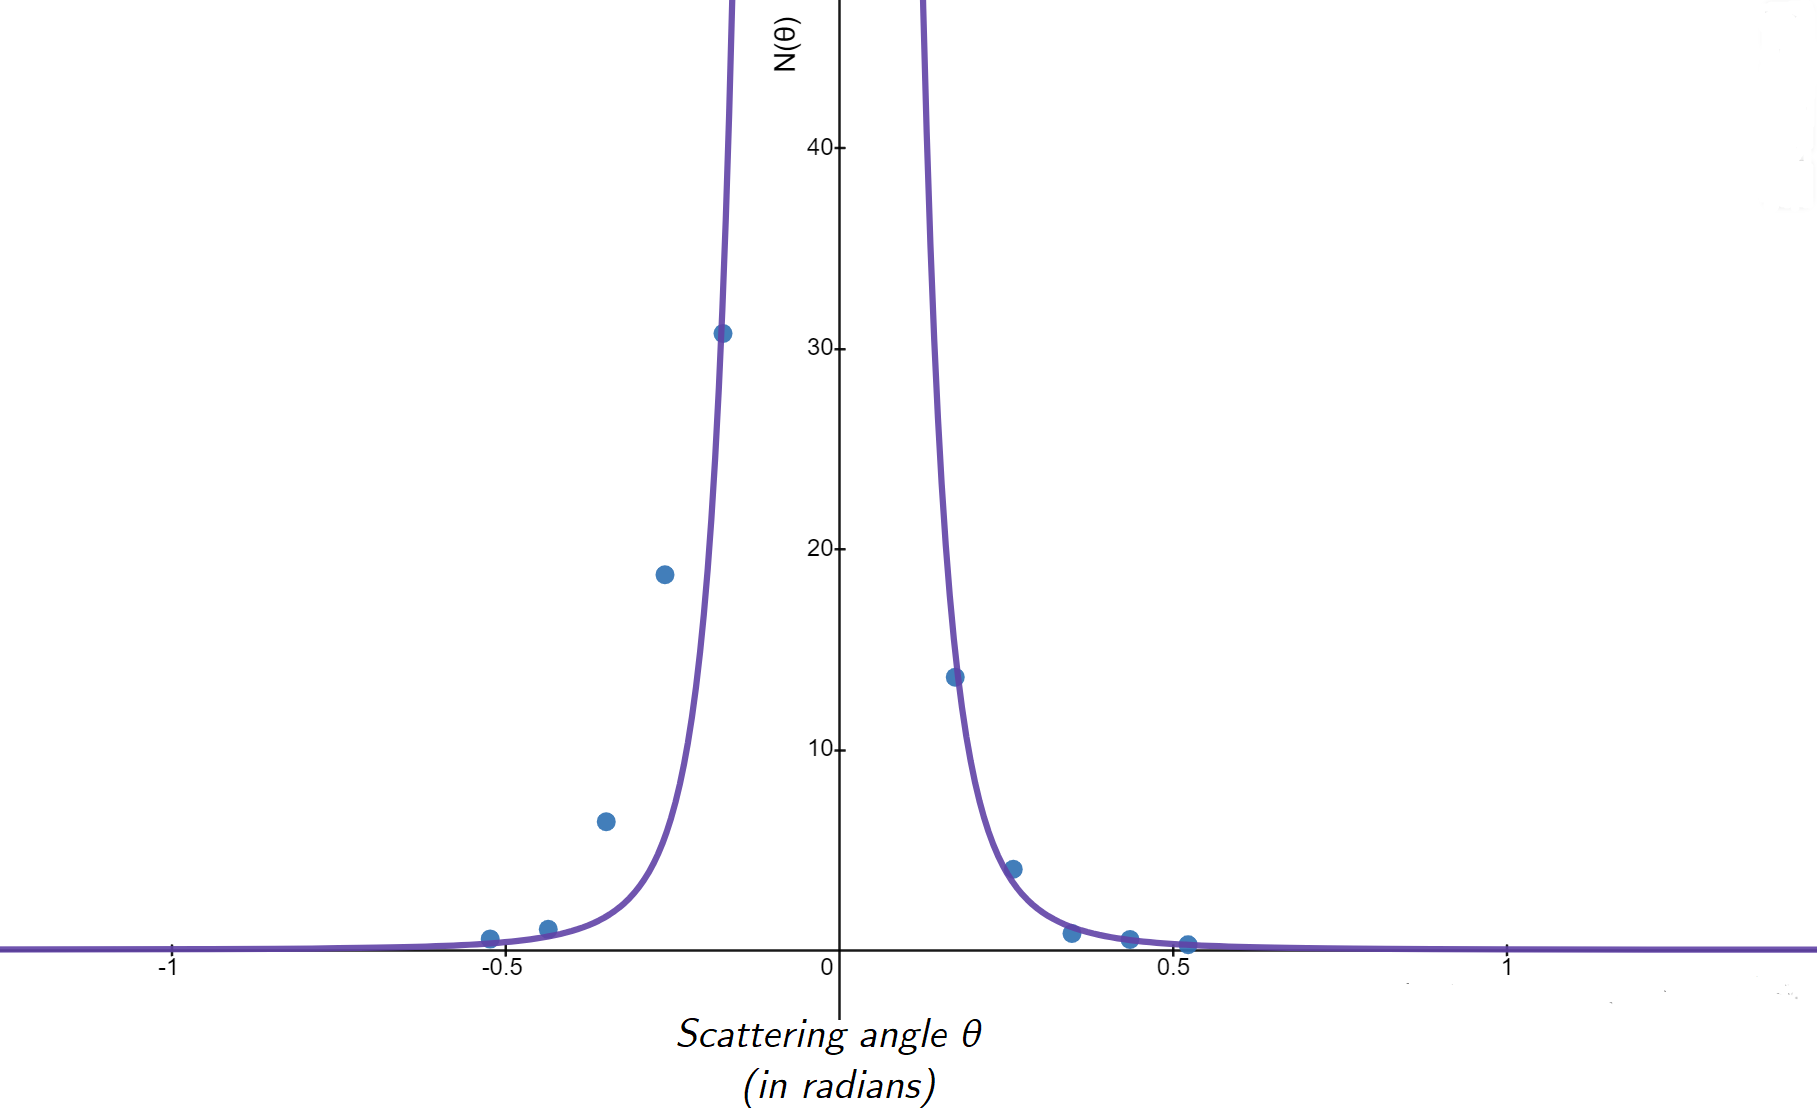
\includegraphics[scale = 0.2]{Figures/graph.png}
        \caption{The plot of scattering angle $\theta$ against $N(\theta)$ and the corresponding fitted curve according to equation (\ref{eq:Ntheta})}
        \label{fig:graph}
    \end{figure}
    \begin{table*}[!ht]
    \caption{Measured values for Aluminium foil and slit width $d = \SI{5}{\milli \metre}$}
    \label{tab:data}
    
    \begin{tabular}{@{}ccccccc@{}}
    \toprule
    \begin{tabular}[c]{@{}c@{}}\textbf{Angle}, $\theta$\\ (degrees)\end{tabular} & \begin{tabular}[c]{@{}c@{}}\textbf{Angle}, $\theta$\\ (radians)\end{tabular} & \begin{tabular}[c]{@{}c@{}}\textbf{Gate time} $t(\theta)$\\ ($s$)\end{tabular} & \textbf{Pulse counts} $n(\theta)$ & \begin{tabular}[c]{@{}c@{}}\textbf{Mean Pulse counts}\\ $n_m(\theta)$ \end{tabular} & \begin{tabular}[c]{@{}c@{}}\textbf{Counting rate} \\ \textit{(directly)} \\ $N_d (\theta)$ ($\si{\per \second}$)\end{tabular} & \begin{tabular}[c]{@{}c@{}}\textbf{Counting rate} \\ \textit{(space corrected)} \\ $N (\theta)$ ($\si{\per \second}$)\end{tabular} \\ \midrule \\
    
    -15                                                      & -0.262                                                         & 1000                                                     & 2092         & 2092                                                                 & 2.092                                                              & 3.402                                                                            \\ \\
    15                                                       & 0.262                                                          & 1000                                                     & 175         & 175                                                                 & 0.175                                                              & 0.285                                                                            \\ \\
     \bottomrule
    \end{tabular}
    \end{table*}
    
\section{Discussions}
    \begin{enumerate}
        \item A small inaccuracy of the collimator-slit adjustment or non-centric distribution of the radiation, coming from the preparation in the holder, may cause a shift of the curve along the horizontal axis (angle shift $<3 \degree$).
        \item Due to such effects it is useful to record scattering rates as well in the positive as in the negative angular range, to get information of both branches with respect to an accurate determination of the symmetry-axis displacement.
    \end{enumerate}

\section{Precautions}
    \begin{enumerate}
        \item The radioactive sources should be held with utmost care.
        \item Never touch the gold or aluminium foil.
        \item Venting of the chamber after the experiment has to be done very carefully.
    \end{enumerate}
\section{Conclusions}
    The results obtained through the experiment were satisfactory and as expected.






\end{document}
%
% ****** End of file apssamp.tex ******
